% Copyright 2004 by Till Tantau <tantau@users.sourceforge.net>.
%
% In principle, this file can be redistributed and/or modified under
% the terms of the GNU Public License, version 2.
%
% However, this file is supposed to be a template to be modified
% for your own needs. For this reason, if you use this file as a
% template and not specifically distribute it as part of a another
% package/program, I grant the extra permission to freely copy and
% modify this file as you see fit and even to delete this copyright
% notice. 
\documentclass{beamer}
\usepackage[utf8]{inputenc}
\usepackage{booktabs}
\usepackage{multirow}
\usepackage{graphics}
\setbeamertemplate{bibliography item}{[\theenumiv]}

% There are many different themes available for Beamer. A comprehensive
% list with examples is given here:
% http://deic.uab.es/~iblanes/beamer_gallery/index_by_theme.html
% You can uncomment the themes below if you would like to use a different
% one:
%\usetheme{AnnArbor}
%\usetheme{Antibes}
%\usetheme{Bergen}
%\usetheme{Berkeley}
%\usetheme{Berlin}
%\usetheme{Boadilla}
%\usetheme{boxes}
%\usetheme{CambridgeUS}
\usetheme{Copenhagen}
%\usetheme{Darmstadt}
%\usetheme{default}
%\usetheme{Frankfurt}
%\usetheme{Goettingen}
%\usetheme{Ilmenau}
%\usetheme{Luebeck}
%\usetheme{Madrid}
%\usetheme{Malmoe}
%\usetheme{Marburg}
%\usetheme{Montpellier}
%\usetheme{PaloAlto}
%\usetheme{Pittsburgh}
%\usetheme{Rochester}
%\usetheme{Singapore}
%\usetheme{Szeged}
%\usetheme{Warsaw}


%Choose a color theme
%\usecolortheme{default} %blue % Fondo blanco, barras azules
%\usecolortheme{albatross} %invasive % Fondo azul intenso
%\usecolortheme{beaver} %Nice % Fondo blanco, Barras grises, Titulos rojos
%\usecolortheme{beetle} %hard
%\usecolortheme{crane} %god
\usecolortheme{dolphin} %soft and elegant
%\usecolortheme{dove} %monochromatic
%\usecolortheme{fly} %invasive
%\usecolortheme{lily}
%\usecolortheme{orchid} % Simular al default
%\usecolortheme{rose}
%%%%\usecolortheme{seagull} % Fondo blanco, Barras grises
%\usecolortheme{seahorse} %PINK
%\usecolortheme{whale} % Similar al default
%\usecolortheme{wolverine} % Fondo blanco, Barras amarillas
% for large table of contents

%% Se customizan colores del tema:
\definecolor{myblue1}{RGB}{17,44,83}
\definecolor{myblue2}{RGB}{32,81,153}
\setbeamercolor{structure}{fg=myblue1, bg=white}

\setbeamercolor{section in head/foot}{fg=white,   bg=myblue1}
\setbeamercolor{subsection in head/foot}{fg=white,bg=myblue2}

\makeatletter
\def\beamer@tocaction@only#1{\only<.(1)>{\usebeamertemplate**{#1}}}
\define@key{beamertoc}{subsectionsonly}[]{\beamer@toc@subsectionstyle{show/only}\beamer@toc@subsubsectionstyle{show/shaded/hide}}
\makeatother


\title{TITULO GENERAL}

% A subtitle is optional and this may be deleted
\subtitle{Subtitulo del trabajo}

\author{David Valenzuela Urrutia\inst{1} \inst{2}}
% - Give the names in the same order as the appear in the paper.
% - Use the \inst{?} command only if the authors have different
%   affiliation.

\institute[GeoInnova Consultores Ltda.] % (optional, but mostly needed)
{
  \inst{1}%
  M.Sc.Electrical Engineering\\
  Universidad de Chile.
  \and
  \inst{2}%
    Ingeniero de proyectos I+D\\ 
    GeoInnova}
% - Use the \inst command only if there are several affiliations.
% - Keep it simple, no one is interested in your street address.

\date{Presentación 1,    24 de Febrero 2017.}
% - Either use conference name or its abbreviation.
% - Not really informative to the audience, more for people (including
%   yourself) who are reading the slides online

\subject{Data Science}
% This is only inserted into the PDF information catalog. Can be left
% out. 

% If you have a file called "university-logo-filename.xxx", where xxx
% is a graphic format that can be processed by latex or pdflatex,
% resp., then you can add a logo as follows:

% \pgfdeclareimage[height=0.5cm]{university-logo}{university-logo-filename}
% \logo{\pgfuseimage{university-logo}}

% Delete this, if you do not want the table of contents to pop up at
% the beginning of each subsection:
\AtBeginSection[]
{
  \begin{frame}[shrink]{$~$}
  %hidesubsections
    \tableofcontents[currentsection, hidesubsections]
  \end{frame}
}

% Agrega el numero de página actual y el número de página global
\addtobeamertemplate{navigation symbols}{}{%
    \usebeamerfont{footline}%
    %\usebeamercolor[fg]{footline}%
    \usebeamercolor[black]{footline}%
    \hspace{1em}%
    \insertframenumber/\inserttotalframenumber
}


% Let's get started
\begin{document}

\begin{frame}
  \titlepage
\end{frame}



\begin{frame}[shrink]{$~$}
  \tableofcontents[hideallsubsections, subsectionsonly, pausesections]
  % You might wish to add the option [pausesections]
\end{frame}



% Section and subsections will appear in the presentation overview
% and table of contents.


\section{Introducción}

\subsection{Subsection 1 Introducción.}
\begin{frame}{Subsection 1 Introducción.}
  \begin{itemize}
  \item Item 1:\\
  \textit{"Texto ..."}
  \pause
    \item Item 2.
  \pause
  \item Item 3.

  \end{itemize}

\end{frame}



\subsection{Subsection 2 Introducción.}
\begin{frame}{Subsection 2 Introducción.}

  \begin{itemize}
      \item Item 1.
      \item Item 2.
      \item Item 3.
      \item Item 4.
      \item Item 5.
  \end{itemize}
\end{frame}


\section{Desarrollo 1}

\subsection{Subsection 1 Desarrollo 1}
\begin{frame}{Subsection 1 Desarrollo 1}{Subtitulo de subsection:}
Según Christopher M. Bishop\cite{C.Bishop}:
\vspace{0.5 cm}

\centering{\textit{"El campo del reconocimiento de patrones se refiere al descubrimiento automático de regularidades en datos mediante el uso de algoritmos computacionales y usar estas regularidades para tomar acciones tales como clasificar los datos en diferentes categorías."}}
\end{frame}


\begin{frame}{Titulo 1 dentro de la subsección:}
  \begin{itemize}
      \item Item 1.
      \item Item 2.
      \item Item 3.
      \item Item 4.
  \end{itemize}
\end{frame}


\begin{frame}{Titulo 2 dentro de la subsección:}
\begin{figure}
    
\includegraphics[scale=0.2]{figura1.png}
    \caption{Figura 1.}
\end{figure}  
\end{frame}

% [shrink] autoajusta el tamaño del contenido
\begin{frame}[shrink]{Titulo 3 dentro de la subsección:} 
\begin{itemize}
    \item Item 1.
    \item Item 2.
    \item Item 3 $\{\vec{X}_{i}, \vec{Y}_{i}\}_{i=1}^{N}$.
\end{itemize}
\end{frame}

\subsection{Subsection 2}
\begin{frame}{Subsection 2}
\begin{itemize}
    \item Item 1.
    \item Item 2.\cite{CVision}
    \item Item 3.
\end{itemize}
\end{frame}


\subsection{Subsection 3}
\begin{frame}{Subsection 3}{Subsection 3 subtitulo}
Contenido de texto ...
\pause
\begin{figure}[H]
    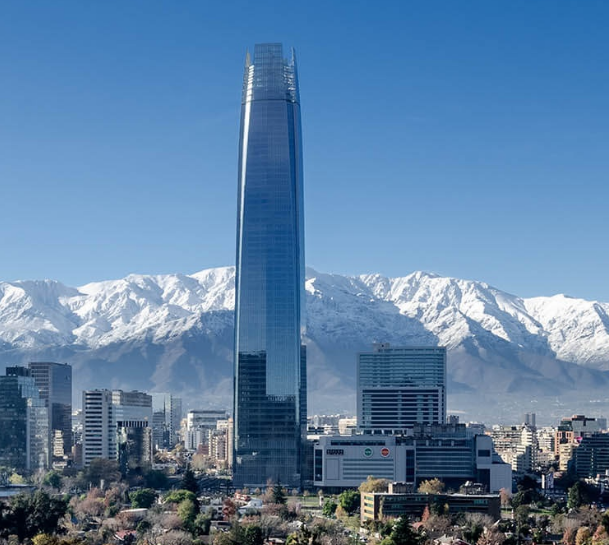
\includegraphics[scale=0.2]{figura2.png}
    \caption{Figura número 2}
\end{figure}
\end{frame}


\begin{frame}{Titulo 1 en subsection 3}{subtitulo ...}
\begin{itemize}
    
\item Item 1.
\item Item 2.
\begin{equation}
    y = f\left (\sum_{i=1}^{N} W_{i}*X_{i} + b \right)
\end{equation}
\end{itemize}
\end{frame}


\begin{frame}{Titulo 2 en subsection 3}{subtitulo ...}
    \begin{figure}[H]
        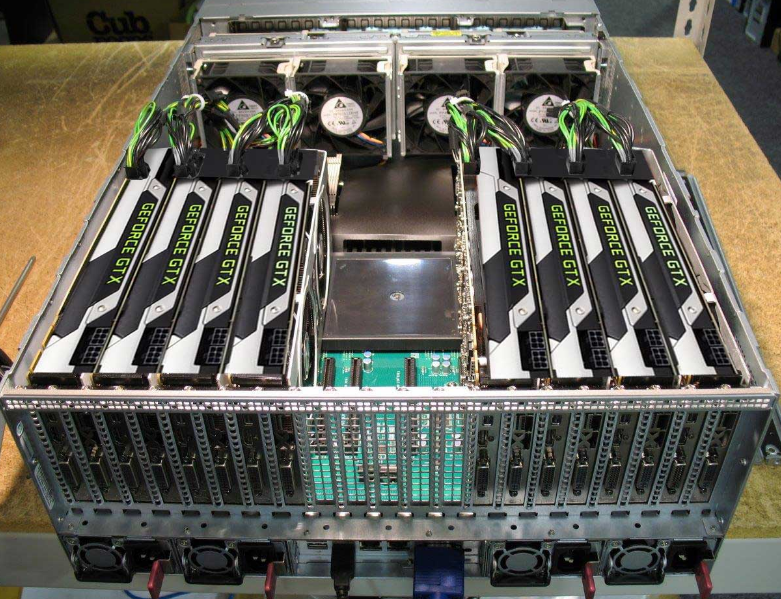
\includegraphics[scale=0.3]{figura3.png}
    \end{figure}
\end{frame}


\begin{frame}
Esta nueva slide no tiene titulo.

\begin{enumerate}
    \item Item 1.
    \item Item 2.
    \item Como ingresar una URL: \url{http://www.nature.com}
\end{enumerate}

\end{frame}


\subsection{Subsection 4}
\begin{frame}{Subsection 4}{subtitulo ...}
\begin{figure}[H]
    
\includegraphics[scale=0.3]{figura4.png}
    \caption{Pie de imagen.}
\end{figure}
\end{frame}


\subsection{Subsection 5}
\begin{frame}{Subsection 5}

Texto de introducción.

\center{\textbf{Texto en negritas y centrado.}}
\pause
\begin{enumerate}
    \item Item 1.
    \item Item 2.
\end{enumerate}
\end{frame}


\section{Section 3}

\subsection{Section 3 - Subsection 1}
\begin{frame}{Section 3 - Subsection 1 - Titulo 1}{Subtitulo 1}
    \begin{itemize}
        \item Item 1.
        \item Item 2.
    \end{itemize}
\end{frame}

\begin{frame}{Section 3 - Subsection 1 - Titulo 2}{Subtitulo 2}
\begin{itemize}
    \item Item 1:
    \begin{enumerate}
        \item Item 1.1.
        \item Item 1.2.
    \end{enumerate}
    \item Item 2.
\end{itemize}
\end{frame}


\begin{frame}
  \begin{table}[H]
\centering
\caption{Esta es la tabla Nº 1.}
\begin{tabular}{@{}lll@{}}
\toprule
Zona     & Imágenes & Porcentaje \\ \midrule
A        & 1831     & 60,07      \\
B        & 557      & 18,27      \\
C        & 660      & 21.65      \\
Total    & 3048     & 100        \\ \bottomrule
\end{tabular}
\end{table}

\end{frame}    

\begin{frame}
\begin{table}[H]
\centering
\caption{Esta es una tabla más compleja}
\label{my-label}
\scalebox{0.42}{
\begin{tabular}{@{}lllllll@{}}
\toprule
\textit{\begin{tabular}[c]{@{}l@{}}Tipo       \\ (Macro-clase)\end{tabular}} & \textit{Cantidad} & \textit{Porcentaje} & \textit{\begin{tabular}[c]{@{}l@{}}Micro-clase\\ (Abundancia)\end{tabular}} & \textit{Cantidad} & \textit{\begin{tabular}[c]{@{}l@{}}Porcentaje en\\ macro clase\end{tabular}} & \textit{\begin{tabular}[c]{@{}l@{}}Porcentaje en\\ micro clase\end{tabular}} \\ \midrule
\multirow{3}{*}{A} & \multirow{3}{*}{128} & \multirow{3}{*}{6,6} & Débil & 38 & 1,97\% & 29,69\% \\ \cmidrule(l){4-7} 
 &  &  & Moderado & 31 & 1,61\% & 24,22\% \\ \cmidrule(l){4-7} 
 &  &  & Fuerte & 59 & 3,06\% & 46,09\% \\ \midrule
\multirow{3}{*}{B} & \multirow{3}{*}{308} & \multirow{3}{*}{15,95} & Débil & 24 & 1,24\% & 7,79\% \\ \cmidrule(l){4-7} 
 &  &  & Moderado & 91 & 4,72\% & 29,55\% \\ \cmidrule(l){4-7} 
 &  &  & Fuerte & 193 & 10,00\% & 62,66\% \\ \midrule
\multirow{3}{*}{C} & \multirow{3}{*}{99} & \multirow{3}{*}{5,12} & Débil & 18 & 0,93\% & 18,18\% \\ \cmidrule(l){4-7} 
 &  &  & Moderado & 43 & 2,23\% & 43,43\% \\ \cmidrule(l){4-7} 
 &  &  & Fuerte & 38 & 1,97\% & 38,38\% \\ \midrule
\multirow{3}{*}{D} & \multirow{3}{*}{403} & \multirow{3}{*}{20,88} & Débil & 12 & 0,62\% & 2,98\% \\ \cmidrule(l){4-7} 
 &  &  & Moderado & 183 & 9,48\% & 45,41\% \\ \cmidrule(l){4-7} 
 &  &  & Fuerte & 208 & 10,78\% & 51,61\% \\ \midrule
\multirow{3}{*}{\begin{tabular}[c]{@{}l@{}}E \\ (E inferior)\end{tabular}} & \multirow{3}{*}{982} & \multirow{3}{*}{50,88} & Débil & 159 & 8,24\% & 16,19\% \\ \cmidrule(l){4-7} 
 &  &  & Moderado & 307 & 15,91\% & 31,26\% \\ \cmidrule(l){4-7} 
 &  &  & Fuerte & 516 & 26,74\% & 52,55\% \\ \midrule
\begin{tabular}[c]{@{}l@{}}F\\ (F inferior)\end{tabular} & 10 & 0,51 & - & - & 0,52\% &  \\ \midrule
\textbf{Total} & \textbf{1930} & \textbf{100,00\%} & \textbf{-} & \textbf{1930} & \textbf{100,00\%} &  \\ \bottomrule
\end{tabular}}
\end{table}
\end{frame}


\subsection{Section 3 - Subsection 2}


\begin{frame}{Section 3 - Subsection 2 - Titulo 1}
  \begin{itemize}
  \item \textbf{Item 1:} Contenido Item 1.
  \item \textbf{Item 2:} Contenido Item 2.
  \begin{enumerate}
      \item Punto 1.
      \item Punto 2.
      \item Punto 3.
      \item Punto 4.
      \pause
  \end{enumerate}

  \end{itemize}
\end{frame}

\subsection{Section 3 - Subsection 3}
\begin{frame}{Section 3 - Subsection 3 - Titulo 1}
\begin{itemize}
    \item Item 1.
    \item Item 2.
\end{itemize}
\end{frame}

\begin{frame}{Section 3 - Subsection 3 - Titulo 2}
  \begin{itemize}
      \item Item 1.
      \item Item 2.
      \item Item 3.
  \end{itemize}
\end{frame}

\section{Section 4}
\begin{frame}{Section 4}{Subtitulo}

\begin{itemize}
    \item Item 1
    \begin{enumerate}
        \item Enum 1.
        \item Enum 2.
    \end{enumerate}
    \item Item 2.
\end{itemize}
\end{frame}

\subsection{Section 4 - subsection 1}
\begin{frame}{Section 4 - subsection 1 - Titulo 1}{subtitulo}
\begin{itemize}
    \item Item 1.
    \item Item 2.
\end{itemize}
\end{frame}

\subsection{Section 4 - subsection 2}
\begin{frame}{Section 4 - subsection 2}{subtitulo}
  \begin{itemize}
      \item Item 1.
      \item Item 2.
  \end{itemize}
\end{frame}

\subsection{Section 4 - subsection 3}
\begin{frame}{Section 4 - subsection 3}

Texto introductiorio ... :

\begin{itemize}
\item \textbf{Item 1} Item 1.
\item \textbf{Item 2} Item 2.
\item \textbf{Item 3} Item 3.
\end{itemize}
\end{frame}


% Placing a * after \section means it will not show in the
% outline or table of contents.

% All of the following is optional and typically not needed.
\section{Referencias}
\begin{frame}[shrink]{Referencias}
  \begin{thebibliography}{10}
    
   %\beamertemplatebookbibitems
  % Start with overview books.

  \bibitem{C.Bishop}
  \emph{Nombre titulo 1}, Autor1.
  
  \bibitem{CVision}
  \emph{Nombre titulo 2}, Autor2.
    
  \bibitem{fukushima}
  \emph{Nombre titulo 3}, Autor3.

  \end{thebibliography}
\end{frame}


\end{document}